\def\assignmenttitle{Modelling and Predicting the Number of Airline Passengers}
\def\assignmentnumber{3}
\def\assignmentdate{29-10-2011}

\documentclass[11pt]{article}
\linespread{1}

\renewcommand{\thefootnote}{\fnsymbol{footnote}}

\usepackage{geometry} % see geometry.pdf on how to lay out the page. There's lots.
\usepackage[utf8]{inputenc}
\usepackage{array}
\usepackage{amsmath,amssymb,latexsym,epic,eepic,epsfig,graphics,psfrag}
\usepackage{amsfonts}
\usepackage{graphicx,float}

\usepackage[danish]{babel}

\usepackage[bottom]{footmisc}

\usepackage{fancyhdr}
\pagestyle{fancy}
\lhead{\small\textit{01246 Partial Differential Equations - Fall 2011 - Anders Hørsted (s082382)}}
\rhead{\thepage}
\chead{}
\lfoot{}\cfoot{}\rfoot{}

\usepackage{pstricks}
\usepackage{pst-node}
\usepackage{wrapfig}
\usepackage{caption}
\usepackage{multirow}
%\usepackage{fouriernc}
%\usepackage[charter]{mathdesign}
\usepackage{lmodern}
\usepackage[normalem]{ulem}
\geometry{a4paper} % or letter or a5paper or ... etc
% \geometry{landscape} % rotated page geometry

\usepackage{subfigure}
\usepackage{placeins}
\usepackage{url}
\usepackage{natbib}
\renewcommand\bibsection*{}
\bibliographystyle{plain}

\makeatletter
\renewcommand*\env@matrix[1][*\c@MaxMatrixCols c]{%
  \hskip -\arraycolsep
  \let\@ifnextchar\new@ifnextchar
  \array{#1}}
\makeatother

\newcommand\myimp{\quad\Leftrightarrow\quad}
\newcommand\half{\frac{1}{2}}
%\newcommand\myvec[1]{\mathbf{#1}}
\newcommand\myvec[1]{\boldsymbol{#1}}
\newcommand\vecx{\myvec{x}}
\newcommand\mymod[1]{\ (\text{mod }#1)}
\newcommand\myreal{\mathbb{R}}
\newcommand\mynatural{\mathbb{N}}
\newcommand\myinteger{\mathbb{Z}}
\newcommand\mycomplex{\mathbb{C}}
\newcommand\myint{\text{int}}
\newcommand\norm[1]{||\,#1\,||}
\newcommand\bignorm[1]{\big|\big|\,#1\,\big|\big|}
\newcommand\seq[1]{\big\{#1\big\}}
\newcommand\smallseq[1]{\{#1\}}
\newcommand\smallseqtoinf[1]{\smallseq{#1}_{k=1}^\infty}
\newcommand\lonew{\ell^1_w}
\newcommand\lone{\ell^1}
\newcommand\ltwo{\ell^2(\mynatural)}
\newcommand\ip[2]{\langle#1,#2\rangle}
\newcommand\hilbert[1]{\mathcal{#1}}
\newcommand\uinf{u_{\infty}}
\newcommand\erf{\text{erf\,}}
\newcommand\infint{\int_{\infty}^{\infty}}
\newcommand\celsius{$^\circ$C}
\newcommand\comsol{Comsol}
\newcommand\fourier{\mathcal{F}}

\usepackage{tabulary}
\newcolumntype{y}{>{\centering\arraybackslash}R}

\setlength{\unitlength}{2mm}
\usepackage{tikz}

\title{Homework \homeworknumber}
\author{01246 Partial differential equations -- \homeworkdate -- Anders Hørsted (s082382)}
%\author{}
\date{} % delete this line to display the current date


%%% BEGIN DOCUMENT
\begin{document}

\maketitle


In this report a model of the monthly number of airline passengers in the U.S.
is build. The data set used to build the model is the actual number of
passengers for every month between January 1995 and March 2002. To be able to
give an estimate of the precision of the model, the data set is separated into
two parts: A training set containing data for the period January 1995 to June
2001, and a test set containing data for the period July 2001 to March 2002.
Throughout the modelling phase we work as if only the training set is
available. The test set is used when the final model have been build, to
compare the predictions of the final model, and the actual numbers in the test
set. From now and until the section about measuring the model performance the
training set is just referred to as ``the data set'' or ``the data''


\section*{Data exploration}

In this section the data set is introduced. First a plot of the data is created
and shown in figure~\ref{fig:trainingset}. \par

\begin{figure}[ht]
\centering
\includegraphics[width=120mm]{../plots/trainingset.pdf}
\caption{Plot of data set used for modelling}
\label{fig:trainingset}
\end{figure}

From the plot a general upward trend is recognized. This isn't surprising since
the U.S. economy got stronger (REFERENCE!!!) in the period and therefore more
airline passengers should be expected. Also a regular seasonal pattern can be
seen which isn't surprising either. In the summer months e.g. we would expect
more passengers than for the other months etc. The conclusion of these two
observations is that the time series is non-stationary and this is something
that should be coped with during the modelling phase. To support that the time
series is non-stationary the estimated autocorrelation function (\acf) and partial
autocorrelation function (\pacf) are now plotted (see
figure~\ref{fig:acfs-trainingset}) \par

\begin{figure}[ht]
    \centering
    \mbox{  
        \subfigure{\includegraphics[width=70mm]{../plots/acf-trainingset.pdf}} \quad 
        \subfigure{\includegraphics[width=70mm]{../plots/pacf-trainingset.pdf}} 
    }
    \caption{CAPTION!!!}
    \label{fig:acfs-trainingset}
\end{figure}

Neither the \acf\ or the \pacf\ are decreasing fast toward zero which further confirms that the time serie is non-stationary (REFERENCE!!!).


\section*{Building the model}

It is time to start building the model. Since the time series is non-stationary a natural first step is to take the first order difference of the series. With $Y_t$ the original series a new series is defined as

\begin{equation*}
    W_t = \nabla Y_t
\end{equation*}

The \acf\ and \pacf\ are calculated for this new series and are shown in figure~\ref{fig:acfs-onediff}. \par

\begin{figure}[ht]
    \centering
    \mbox{  
        \subfigure{\includegraphics[width=70mm]{../plots/acf-onediff.pdf}} \quad 
        \subfigure{\includegraphics[width=70mm]{../plots/pacf-onediff.pdf}} 
    }
    \caption{CAPTION!!!}
    \label{fig:acfs-onediff}
\end{figure}

From the \acf\ of the differenced series it is seen that the estimated
correlation for most lags are not significantly different from zero, except for
the lags 6, 12, 18, 24. Also lag 6 and 18 are negative and 12 and 24 is
positive. This confirms the 12-period seasonality that was observed in the plot
of the original time series. A natural next step is therefore to do a seasonal
differencing giving a new series as

\begin{align*}
    Z_t &= \nabla_{12}W_t \\
    &= \nabla\nabla_{12}Y_t
\end{align*}

The \acf\ and \pacf\ of the new series are shown in figure~\ref{fig:acfs-seasondiff}. \par

\begin{figure}[ht]
    \centering
    \mbox{  
        \subfigure{\includegraphics[width=70mm]{../plots/acf-seasondiff.pdf}} \quad 
        \subfigure{\includegraphics[width=70mm]{../plots/pacf-seasondiff.pdf}} 
    }
    \caption{CAPTION!!!}
    \label{fig:acfs-seasondiff}
\end{figure}

It is seen that most lags of the \acf is zero, except for lag 1 and 12. For the \pacf\ the lags 1, 2, 6 and 11 are different from zero. Based on this it looks as if it is possible to model the original series $Y_t$ as a multiplicative $(p,1,q)\times(P,1,Q)_{12}$ seasonal model. Since only lag 1 and 12 are different from 0 in the \acf\ a model with $q=1$ and $Q=1$, could be tried. Ignoring lag 6 and 11 in the \pacf\ for now $p=2$ and $P=0$ is attempted.

\subsection*{The $(2,1,1)\times(0,1,1)_{12}$ seasonal model}

Using the \myverb{arima} function in R a $(2,1,1)\times(0,1,1)_{12}$ seasonal model is now fitted to the original time series. The resulting model is given by \par

\begin{align*}
    (1 + 0.20B + 0.27B^2)(1-B)(1-B^{12})Y_t &= (1-0.40B)(1-0.46B^{12})\varepsilon_t \myimp\\
    (1 + 0.20B + 0.27B^2)Z_t &= (1-0.40B)(1-0.46B^{12})\varepsilon_t
\end{align*}

To check the model the residuals are checked to see if they resemble white noise as they should for an adequate model. First the residuals are plotted and a QQ-plot of the residuals are also created. Both are shown in figure~\ref{fig:qq-residuals-m1}. \par

\begin{figure}[htb]
    \centering
    \mbox{
        \subfigure{\includegraphics[width=70mm]{../plots/residuals-m1.pdf}} \quad 
        \subfigure{\includegraphics[width=70mm]{../plots/qq-residuals-m1.pdf}}
    }
    \caption{CAPTION!!!}
    \label{fig:qq-residuals-m1}
\end{figure}

From both plots it looks as if the residuals are pretty close to white noise. Doing a sign test on the residuals gives a p-value of 0.27 which also supports that the residuals are white noise. Also the \acf\ for the residuals is plotted and shown in figure~\ref{fig:acf-m1} \par

\begin{figure}[htb]
    \centering
    \includegraphics[width=70mm]{../plots/acf-m1.pdf}
    \caption{CAPTION!!!}
    \label{fig:acf-m1}
\end{figure}

The \acf\ also support that the residuals are white noise, since only lag 0 is different from 0. By all means it looks as if the chosen model is able to describe the original time series and so it only remains to check whether a simpler model exists that explains the data just as well. From the estimated parameters of the model along with the standard error of the estimates (see figure~\ref{fig:coeffs-m1}) it looks as if at least some of the parameters are redundant and it is expected that a simpler model exists. The primary candidate for changes is the normal AR(2)-part of the model which could possible be changed to 0 or 1. Therefore a $(0,1,1)\times(0,1,1)_{12}$ model is now tested.

\begin{figure}[ht]
    \centering
    \parbox{.48\textwidth}{\lstinputlisting[firstline=6,lastline=9]{../tables/model1.txt}}
    \caption{CATION!!!}
    \label{fig:coeffs-m1}
\end{figure}

\subsection*{The $(0,1,1)\times(0,1,1)_{12}$ seasonal model}

Parameters for the $(0,1,1)\times(0,1,1)_{12}$ seasonal model is now estimated from the original time series which gives 

\begin{align*}
    (1-B)(1-B^{12})Y_t &= (1-0.66B)(1-0.45B^{12}) \myimp\\
    Z_t &= (1-0.66B)(1-0.45B^{12})
\end{align*}

By doing all the same model checks as for the previous model we obtain the results shown in figure~\ref{fig:diagnostics-m2}. \par

\begin{figure}
    \centering
    \mbox{%
        \subfigure{\includegraphics[width=70mm]{../plots/residuals-m2.pdf}} \quad 
        \subfigure{\includegraphics[width=70mm]{../plots/qq-residuals-m2.pdf}}
    }
    \mbox{%
        \subfigure{\includegraphics[width=70mm]{../plots/acf-m2.pdf}} \quad 
        \subfigure{\includegraphics[width=70mm]{../plots/pacf-m2.pdf}} \quad 
    }
    \mbox{%
        \subfigure{\parbox{.3\textwidth}{\lstinputlisting[firstline=6,lastline=9]{../tables/model2.txt}}}
    }
    \caption{CAPTION!!!}
    \label{fig:diagnostics-m2}
\end{figure}

From the plots it seems as if the simpler $(0,1,1)\times(0,1,1)_{12}$ model is also able to explain the model and from the coefficients and their standard errors it looks as if this is as simple as the model can be. To further support that the simpler model is to be preferred the AIC is seen (see appendices \ref{app:summary-m1} and \ref{app:summary-m2}) to be lower for the simpler model. The conclusion is that the $(0,1,1)\times(0,1,1)_{12}$ model with coefficients as in equation (\ref{eq:m2}) is accepted as the best model to describe the data. The final test for the chosen model is to predict 9 months ahead in time and then compare with the actual values.


\section*{Prediction with the $(0,1,1)\times(0,1,1)_{12}$ model}

\textit{Note that in this section the data that in the previous section was just called the data set is now referred to as the training set. The data set with airline passenger numbers for July 2001 to March 2002 is called the test set}.\par 

Predictions for the months July 2001 to March 2002 are now made using the \myverb{predict.Arima} function in R. The method is set to Maximum Likelihood. The predictions are plotted along with the training set data and is shown in figure~\ref{fig:training-and-prediction}.\par

\begin{figure}[ht]
    \centering
    \includegraphics[width=120mm]{../plots/training-and-prediction.pdf}
    \caption{CAPTION!!!}
    \label{fig:training-and-prediction}
\end{figure}

From the figure it looks as if the model is capturing the overall pattern in the series well. Now it is tested how well the model fits the real numbers in the test set. The predictions along with the real numbers from the test is therefore plotted in figure~\ref{fig:test-and-prediction}

\begin{figure}[ht]
    \centering
    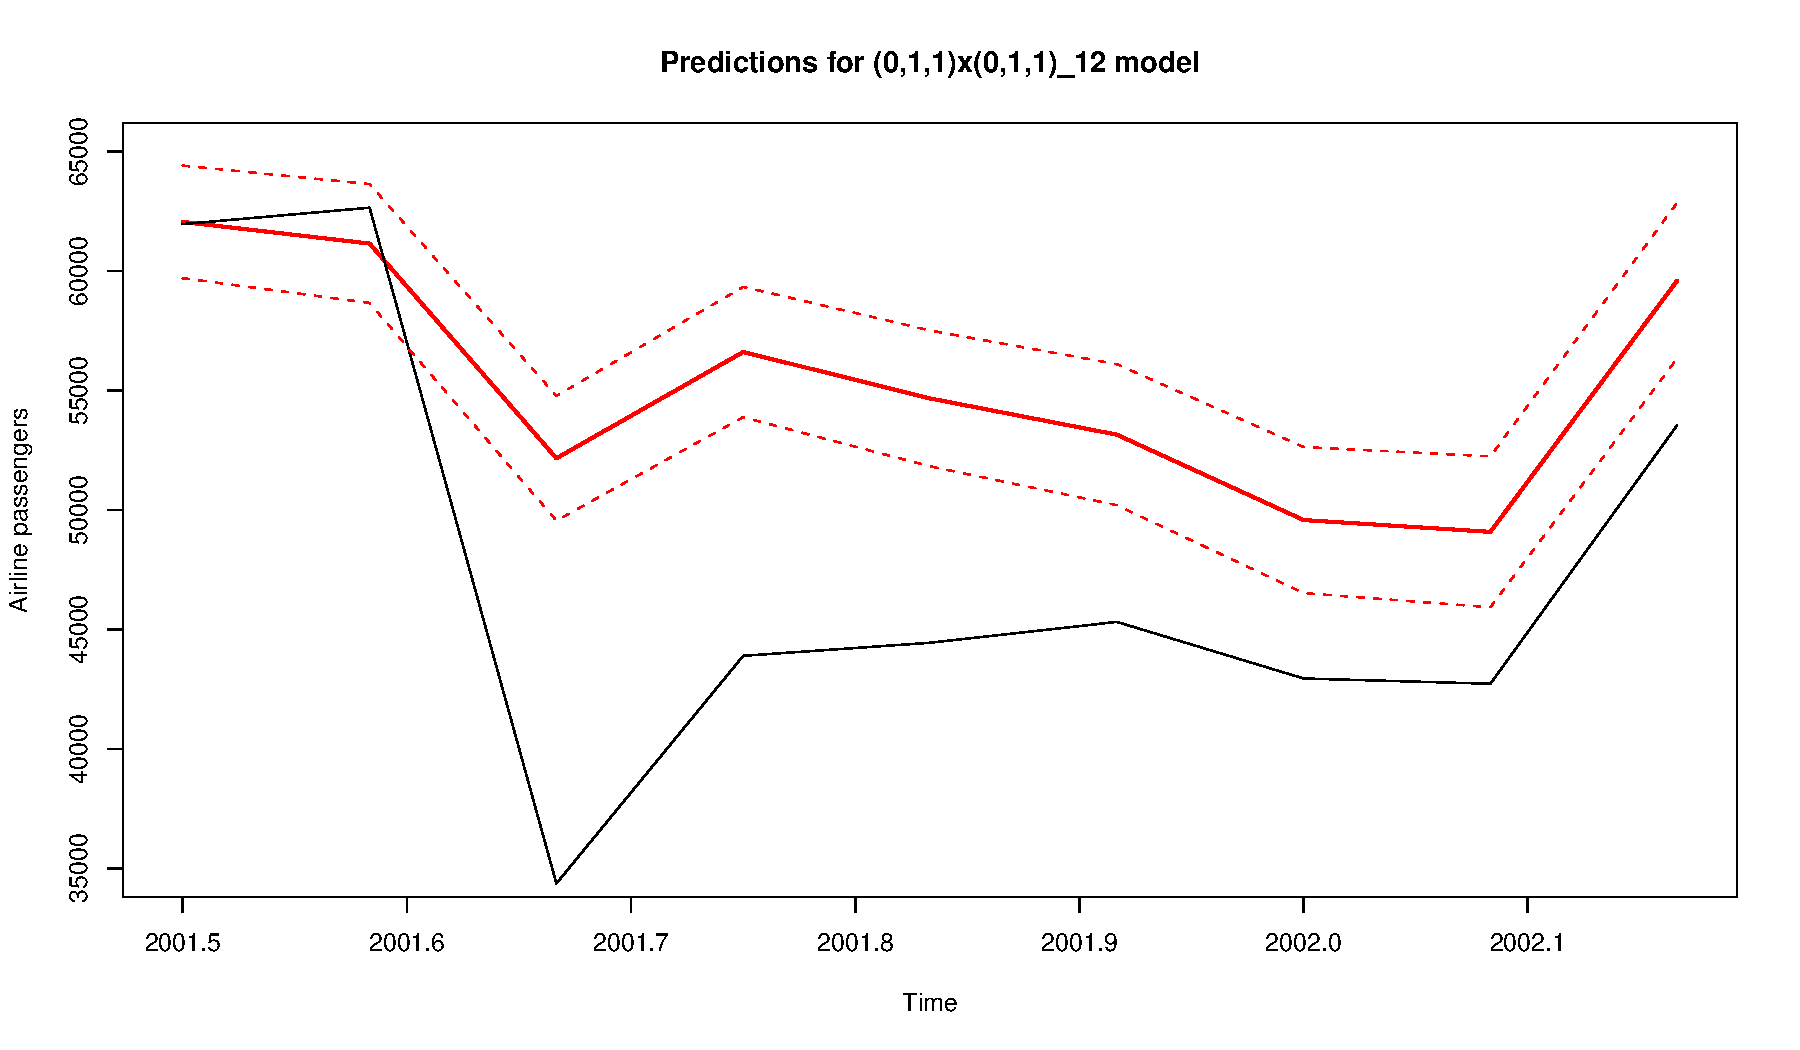
\includegraphics[width=120mm]{../plots/test-and-prediction.pdf}
    \caption{CAPTION!!!}
    \label{fig:test-and-prediction}
\end{figure}

\pagebreak


\renewcommand\thesection{\Alph{section}}
\section{Appendices}

All R code used for this assignment is included here. All source code incl.
latex code for this report can be found at
{\small\url{https://github.com/alphabits/dtu-fall-2011/tree/master/02417/assignment-3}}

\subsection{Load data script}
\lstinputlisting{../src/loaddata.R}

\subsection{Helper functions}
\lstinputlisting{../src/functions.R}

\subsection{Main script}
\lstinputlisting{../src/assignment3.R}

\subsection{Summary for $(2,1,1)\times(0,1,1)_{12}$ model}\label{app:summary-m1}
\lstinputlisting{../tables/model1.txt}

\subsection{Sign test for $(2,1,1)\times(0,1,1)_{12}$ model}
\lstinputlisting{../tables/signtest-m1.txt}

\subsection{Summary for $(0,1,1)\times(0,1,1)_{12}$ model}\label{app:summary-m2}
\lstinputlisting{../tables/model2.txt}

\subsection{Sign test for $(0,1,1)\times(0,1,1)_{12}$ model}
\lstinputlisting{../tables/signtest-m2.txt}

\pagebreak

\begin{thebibliography}{9}

\bibitem{nocedal06}
  Jorge Nocedal \& Stephen J. Wright,
  \emph{Numerical Optimization}.
  Springer Science+Business Media,
  2nd Edition,
  2006.
\bibitem{nielsen10}
  Kaj Madsen \& Hans Bruun Nielsen,
  \emph{Introduction to Optimization and Data Fitting}.
  DTU IMM,
  1st Edition,
  2010.

\end{thebibliography}


\end{document}
